%
\documentclass[12pt]{article}

\usepackage{fullpage}
\usepackage{setspace}
\usepackage{endnotes}
%\usepackage{epsfig}
%\usepackage{psfrag}
\usepackage{amsmath}
\usepackage{amsfonts}
\usepackage{amssymb}
\usepackage{rotating}
\usepackage{dcolumn}
\usepackage{longtable}
\usepackage{microtype}
\usepackage{graphicx}
\usepackage{hyperref}
\usepackage[usenames,dvipsnames]{color}
%\usepackage{hypdvips}
\hypersetup{
 pdftitle={Compression and Conditional Effects}, % title
 pdfauthor={Redacted}, %Carlisle Rainey}, % author
 pdfkeywords={hypothesis testing}{interaction term}{product term}{interaction}{logit} {probit} {logisitic regression}
 pdfnewwindow=true, % links in new window
 colorlinks=true, % false: boxed links; true: colored links
 linkcolor=BrickRed, % color of internal links
 citecolor=BrickRed, % color of links to bibliography
 filecolor=BrickRed, % color of file links
 urlcolor=BrickRed % color of external links
}
\usepackage{url}
\usepackage{natbib}
%\bibpunct{(}{)}{,}{a}{}{;}
\usepackage{framed}
\usepackage{lipsum}
\usepackage[font=small,labelfont=sc]{caption}
 \usepackage{float}
\restylefloat{table}
\bibpunct{(}{)}{;}{a}{}{,}
\newtheorem{lemma}{Lemma}
\newtheorem{proposition}{Proposition}
\newtheorem{theorem}{Theorem}
\newtheorem{claim}{Claim}
\newenvironment{proof}[1][Proof]{\begin{trivlist}
\item[\hskip \labelsep {\bfseries #1}]}{\end{trivlist}}
\newenvironment{definition}[1][Definition]{\begin{trivlist}
\item[\hskip \labelsep {\bfseries #1}]}{\end{trivlist}}
\newenvironment{example}[1][Example]{\begin{trivlist}
\item[\hskip \labelsep {\bfseries #1}]}{\end{trivlist}}
\newenvironment{remark}[1][Remark]{\begin{trivlist}
\item[\hskip \labelsep {\bfseries #1}]}{\end{trivlist}}
%\newcommand{\qed}{\nobreak \ifvmode \relax \else
%      \ifdim\lastskip<1.5em \hskip-\lastskip
%      \hskip1.5em plus0em minus0.5em \fi \nobreak
%      \vrule height0.75em width0.5em depth0.25em\fi}
%      \setlength{\LTcapwidth}{5in}
%\def\p3s{\phantom{xxx}}

\usepackage{tgpagella}
\usepackage[T1]{fontenc}
%\usepackage[T1]{fontenc}
\usepackage[bitstream-charter]{mathdesign}


%Redefine the first level
\renewcommand{\theenumi}{\arabic{enumi}.}
\renewcommand{\labelenumi}{\theenumi}
%Redefine the second level
\renewcommand{\theenumii}{\alph{enumii}.}
\renewcommand{\labelenumii}{\theenumii}
%Redefine the third level
\renewcommand{\theenumiii}{\roman{enumiii}.}
\renewcommand{\labelenumiii}{\theenumiii}
%Redefine the fourth level
\renewcommand{\theenumiv}{\Alph{enumiv}.}
\renewcommand{\labelenumiv}{\theenumiv}


\parskip=0pt
\parindent=20pt
\usepackage{lscape}
\singlespace
\title{Compression and Conditional Effects}
%\author{Carlisle Rainey\thanks{Assistant Professor in the Department of Political Science at the University at Buffalo (SUNY)}}
\date{\today}
\usepackage[normalem]{ulem}

% Create footnote command so that my name
% has an asterisk rather than a one.
\long\def\symbolfootnote[#1]#2{\begingroup%
\def\thefootnote{\fnsymbol{footnote}}\footnote[#1]{#2}\endgroup}

\begin{document}


\begin{center}
\LARGE{\textbf{Compression and Conditional Effects}}\\\vspace{4mm}
\normalsize{\textsc{Carlisle Rainey\symbolfootnote[1]{Thanks to Bill Berry, Scott Clifford, and Justin Esarey for helpful comments on earlier versions of this manuscript.}}}\\\vspace{2mm}
\begin{small}\singlespace
Assistant Professor\\
University at Buffalo (SUNY)\\
Department of Political Science\\
\href{http://www.carlislerainey.com}{carlislerainey.com}\\
\href{mailto:rcrainey@buffalo.edu}{rcrainey@buffalo.edu}\\\vspace{4mm}
For the most recent draft of this manuscript,\\see the project page at \href{http://www.carlislerainey.com/research/compression-and-conditional-effects/}{crain.co/compress}.
\end{small}
\end{center}

\thispagestyle{empty}
%\end{document}
%\newpage
{\centerline{\textbf{Abstract}}}
\begin{quote}\noindent Previous research in political methodology argues that researchers do not need to include a product term in a logistic regression model to test for interaction if they suspect interaction due to compression alone. I disagree with this claim and offer analytical arguments and simulation evidence that when researchers incorrectly theorize interaction due to compression, models without a product term bias the researcher, sometimes heavily, toward finding interaction. However, simulation studies also show that models with a product term fit a broad range of non-interactive relationships surprisingly well, enabling analysts to remove most of the bias toward finding interaction by simply including a product term.\end{quote}
\thispagestyle{empty}
%\newpage
\singlespace
\setcounter{page}{1}

\doublespace

% Introduce the problem

\section*{Introduction}

Many theories in political science suggest an ``interactive'' relationship in which the effect of one explanatory variable $X$ depends on the value of another explanatory variable $Z$. While earlier research lays out a clear and uncontroversial method for testing these claims in the context of linear regression (e.g. \citealt{KamFranzese2007} and \citealt{BramborClarkGolder2006}), political methodologists disagree about the best approach for researchers using logistic regression, particularly over whether a product term must be included in the model (\citealt{Nagler1991}; \citealt{BramborClarkGolder2006}; and \citealt{BerryDeMerittEsarey2010}).\footnote{Throughout the manuscript, I focus on logistic regression models in particular, but the conclusions generalize to a wide range of models of binary outcomes, including probit models.}  

% Provide an overview of previous research 

This debate hinges around the substantive work of \cite{WolfingerRosenstone1980}, who theorize that easing registration restrictions should have a smaller positive effect on the probability of voting among individuals with more education. They do not evaluate the presence of interaction by testing the statistical significance of the product term's coefficient. Indeed, they do not even include a product term in the model. Instead, they simply note that, even without a product term, a logistic regression model can represent the kind of interaction suggested by their theory because the \textit{S}-shaped response curve creates ``compression,'' requiring that all variables have smaller effects as the probability of an event approaches zero or one. 

\begin{quote}\singlespace
As a statistical model, [logistic regression] is a more faithful representation of our substantive theory than [linear regression]. As we will see, the impact of most demographic variables is not constant across all types of individuals. Rather, the effect of a variable depends on the probability that the individual would vote. For example, a high-status occupation or a high-income has less impact on a college graduate who is 90 percent likely to vote, than it has on a high school dropout, who is only 55 percent likely to vote... With [logistic regression] a variable has very little impact on those who are either very unlikely or nearly certain to vote. It has the greatest impact in the middle of the distribution, on those who are between 40 and 60 percent likely to vote and are the most susceptible to the forces pushing them to vote or not to vote (11).
\end{quote}

\noindent Instead of including a product term and testing the statistical significance of its coefficient, \cite{WolfingerRosenstone1980} argue for interaction by calculating a second difference, which is the difference in the effect of easing registration restrictions between individuals with a high and low level of education.\footnote{A second difference $\Delta\Delta$ is the difference in the effect on $\text{Pr}(Y)$ of changing $X$ from a low value to a high value as $Z$ changes from a low value to a high value. Formally, a second difference $\Delta\Delta$ is defined as follows:
\begin{align}
\Delta\Delta &= [\text{Pr}(Y | X = x_{hi}, Z = z_{hi}) - \text{Pr}(Y | X = x_{lo}, Z = z_{hi})]\nonumber \\
&-[\text{Pr}(Y  | X = x_{hi}, Z = z_{lo}) - \text{Pr}(Y  | X = x_{lo}, Z = z_{lo})], \nonumber
\end{align}
where $x_{lo}$, $x_{hi}$, $z_{lo}$, and $z_{hi}$ take on substantively interesting values of the explanatory variables $X$ and $Z$. For more details see \cite{BerryDeMerittEsarey2010}. For a detailed discussion of computing confidence intervals for second differences, see \cite{KingTomzWhittenburg2000}.}  Using this approach, they find, as expected, that easing registration restrictions has a larger effect on the probability of turning out among less educated individuals. 

However, \cite{Nagler1991} rejects this finding because the \textit{S}-shaped curve automatically builds interaction into the model. He claims that ``examining predicted probabilities generated by non-linear models such as [logistic regression] may produce spurious results when used to determine interactive effects between two [explanatory] variables (1393).'' Instead of just calculating a second difference to quantify the amount of interaction, Nagler prefers to argue for interaction by including a product term and testing the statistical significance of its coefficient.  When he does this, the coefficient for the product of education and registration restrictions is incorrectly signed (suggesting that easing restrictions has a larger effect on the propensity to vote among the \textit{most} educated), leading Nagler to conclude that the data do not support Wolfinger and Rosenstone's theory. 

But \cite{BerryDeMerittEsarey2010} (hereafter, BDE) defend Wolfinger and Rosenstone's approach against Nagler's challenge, arguing that ``compression should not be viewed as theoretically irrelevant.'' Instead, they suggest that ``it can be a strong theoretical rationale for expecting interaction between variables in their influence on [the probability of an event] (255).'' Further, BDE suggest that if researchers expect interaction due to compression alone, then ``there is no need to include a product term in the model (261).'' In this situation, BDE recommend following Wolfinger and Rosenstone's strategy of (1) excluding a product term, (2) computing a second difference, and (3) calculating a confidence interval and verifying that it contains only values consistent with the research hypothesis (i.e. is statistically significant). 

Despite compression's theoretical relevance, I argue that researchers should \textit{always} include a product term, even when they expect interaction on the basis of compression alone. A product term is not necessary to allow the model to represent interaction--it can do that with no product term \citep{BerryDeMerittEsarey2010}. A product term must be included because it allows the model to better represent a \textit{non-interactive} relationship. I present an analytical argument and simulations showing that if no product term is included, a logistic regression model cannot represent a non-interactive relationship and thus overstates the evidence for interaction. Fortunately, I find that simply including a product term eliminates most of this bias.
 
\section*{The Argument for Excluding a Product Term}

BDE's overarching claim, which I wholeheartedly agree with, is that ``a statistically significant product term is neither necessary nor sufficient for concluding that there is substantively meaningful interaction among independent variables in their influence on [the probability of an event]'' (261). Given this point though, BDE ask whether it is always necessary to include a product term in the model. To decide whether to include a product term, they suggest that analysts draw a sharp distinction between theories that focus on the unbounded latent variable, denoted as $Y^*$ (perhaps conceptualized as ``utility''), and theories that focus on the probability of an event, denoted as $\text{Pr}(Y)$.\footnote{In BDE's notation, $Y^*$ refers to the so-called ``latent variable'' implied in models of binary outcomes. $Y^*$ simply equals the value of the linear predictor, often denoted by $\eta = X\beta = \beta_0 + \beta_1X_1 + \beta_2X_2 + ... + \beta_kX_k$ in the notation of general linear models, and is transformed into $\text{Pr}(Y)$ by an inverse link function that maps the real line to $[0, 1]$. Sometimes researchers' theories lead to hypotheses about $Y^*$ rather than $\text{Pr}(Y)$. For example, theorists often link formal models of decision-making to random utility models, a common framework for deriving models such as logistic regression, particularly the almost identical probit model. Using this approach, researchers can evaluate explanations relying on utility, represented by the value of $Y^* = \eta = X\beta$.}

\begin{quote}\singlespace
\textit{BDE Recommendation}: The decision to include a product term must be based on an explicit theory about the effects of variables on the unbounded latent dependent variable $Y^*$, assumed by the model.\vspace{2mm}\\
\indent \textit{Part (a)}: If the theory assumes that variables interact in influencing the latent unbounded variable $Y^*$, then the researcher should include a product term.
\end{quote}
\doublespace
We agree on \textit{Part (a)}. As both BDE and \cite{Nagler1991} note, this situation is entirely analogous to linear regression, making a product term essential.
\begin{quote}\singlespace
\indent \textit{Part (b)}: If the theory assumes that variables should interact in influencing $\text{Pr}(Y)$ strictly on an expectation of compression, then there is no need to include a product term in the model.
\end{quote}\doublespace
BDE explain:
\begin{quote}\singlespace 
[I]n any logit or probit model, the marginal effect
of $X$ on $\text{Pr}(Y)$ depends on the values of all [explanatory]
variables; this marginal effect is greatest when $\text{Pr}(Y)$ is
0.5 and declines when a change in either variable pushes
$\text{Pr}(Y)$ toward 0 or 1. We refer to the phenomenon ... as compression,
because deviations of $\text{Pr}(Y)$ away from [0.5] compress
further possible change in \text{Pr}(Y) to ever-smaller ranges.
 (251)
 \end{quote}\doublespace
They continue by suggesting:
\begin{quote}\singlespace
[A] researcher...may base his hypothesis that independent variables interact in influencing $\text{Pr}(Y)$ strictly on an expectation of compression. In this case, there is no need to include a product term in the model. Put differently, no product term is required if the analyst's only reason for positing interaction between $X$ and $Z$ in influencing $\text{Pr}(Y)$ is an expectation that when the value of $X$ is extreme, $\text{Pr}(Y)$ is near its limit of zero or one and thus there is little room for $\text{Pr}(Y)$ to change as $Z$ changes. In any event, the analyst should use the parameter estimates for the model (with no product term) to generate estimates of the effects of variables on $\text{Pr}(Y)$ to test his hypothesis; the same tools used for models with a product term--second differences or marginal effect plots--can be employed.
(261)
\end{quote}
\doublespace


\section*{The Argument for Including a Product Term}

Researchers must employ a statistical model that can represent (1) relationships that are \emph{consistent} with the theory and (2) plausible relationships that are \emph{inconsistent} with the theory. It is obvious that models should be able to represent relationships that are consistent with theory. But if researchers use models that cannot also represent situations \emph{inconsistent} with the theory, then they have assumed their theories are correct. Though the theoretical rationale may be strong, it has not been made vulnerable to the data.

Thus, BDE's analysis is incomplete when they write that ``no product term is required if the analyst's only reason for positing interaction between $X$ and $Y$ in influencing $\text{Pr}(Y)$ is an expectation that when the value of $X$ is extreme, $\text{Pr}(Y)$ is near its limit of zero or one, and thus there is little room for $\text{Pr}(Y)$ to change as $Z$ changes.'' While they correctly note that the theorized relationship can be represented by a model with no product term, they fail to discuss whether this model can also represent relationships that are inconsistent with their theory.

Without a product term, a logistic regression model cannot represent many reasonable situations that are inconsistent with an interactive theory. In particular, it cannot represent a situation in which two explanatory variables have non-zero effects and the probability of an event is greater or less than one-half, but there is no interaction.\footnote{Specifically, for a logistic regression model including $X$ and $Z$, but excluding their product, if all of the following conditions hold, then $X$ and $Z$ must interact in influencing Pr$(Y)$.\footnote{See the intuition of the claim by inspecting the second derivative of Pr($Y$), given by
\begin{center}
$\dfrac{\partial^2 \text{Pr}(Y)}{\partial X \partial Z} = \text{Pr}(Y)[1 - \text{Pr}(Y)][1 - 2\text{Pr}(Y)]\beta_x\beta_z$.
\end{center}
Notice that the second derivative can equal zero if and only if one of the conditions does not hold. For further discussion, see \cite{Nagler1991} and \cite{BerryDeMerittEsarey2010}.}\\
(1.) $X$ has a non-zero effect.\\
(2.) $Z$ has a non-zero effect.\\
(3.) $\text{Pr}(Y) < 0.5$ or $\text{Pr}(Y) > 0.5$.\\This can easily be seen by inspecting the second derivative of the logistical regression model with no product term, given by \begin{align}
\dfrac{\partial^2 \text{Pr}(Y)}{\partial X \partial Z} &=  \text{Pr}(Y)[1 - \text{Pr}(Y)][1 - 2\text{Pr}(Y)]\beta_x \beta_z. \nonumber
\end{align}
If any of 1-3 hold, then the second derivative is exactly zero. Otherwise, the second derivative is non-zero and the model is interactive. Consequentially, if the researcher incorrectly theorizes compression, but 1-3 hold, then a logistic regression model without a product term will overstate the evidence for interaction.\label{fn:conditions}} Therefore, if the researcher incorrectly theorizes compression, a logistic regression model without a product term will likely overstate the evidence for interaction.

With a product term, however, a logistic regression model can represent \textit{some} plausible situations inconsistent with an interactive theory.\footnote{For a logistic regression model including $X$, $Z$, and $XZ$, if all of the conditions (1-3) identified in Footnote \ref{fn:conditions} hold, then $X$ and $Z$ \textit{may or may not} interact in influencing Pr$(Y)$. The intuition of this claim can be seen by simply inspecting the second derivative of a logistic regression model including a product term, given by
\begin{align}
\dfrac{\partial^2 \text{Pr}(Y)}{\partial X \partial Z} &= \text{Pr}(Y)[1 - \text{Pr}(Y)]\beta_{xz} \nonumber\\
&+ \text{Pr}(Y)[1 - \text{Pr}(Y)][1 - 2\text{Pr}(Y)](\beta_x + \beta_{xz}Z )(\beta_z + \beta_{xz}X). \nonumber
\end{align}
The presence of the product term create another coefficient that allows the second derivative to be zero, even if conditions 1-3 hold. Thus, this model is capable of representing situations in which 1-3 hold, but no interaction is present. }
While including a product term does not entirely remove the bias toward confirming interactive hypotheses, it does greatly reduce the bias. Thus, including a product term makes the empirical argument more compelling by making the theory more vulnerable to the data.

\section*{Simulations}

To illustrate the potential consequences of excluding a product term, I report two simulation studies. The first examines a single relationship in detail. The second looks at a wide range of potential relationships. Because I am particularly interested in what happens if the theory (or researcher's hypothesis) is wrong, I imagine that a researcher incorrectly theorizes interaction due to compression and follows BDE's suggestion to exclude the product term. In almost all cases, excluding the product term biases the researcher toward finding support for her theory.

\subsection*{Study \#1: A Fixed Relationship} 

I first consider the non-interactive relationship (i.e. data-generating process) $\text{Pr}(Y) = 0.3 + 0.2X - 0.3Z$ shown in the left panel of Figure \ref{fig:relationships_fits}. I imagine that the analyst correctly suspects that $X$ has a positive effect on $\text{Pr}(Y)$ and $Z$ has a negative effect on $\text{Pr}(Y)$.  She also theorizes that because the event is relatively rare and $Z$ pushes $\text{Pr}(Y)$ even closer to zero,  there is less room for $X$ to affect $\text{Pr}(Y)$. Therefore, she expects that $X$ should have a smaller effect when $Z=1$. But this hypothesis is not correct--she \textit{incorrectly} expects that $X$ and $Z$ interact in influencing $\text{Pr}(Y)$ due to compression. Still, she notices that a logistic regression model can represent the kind of interaction suggested by her theory and decides that no product term is necessary \citep{BerryDeMerittEsarey2010}. 

Because $X$ is approximately uniformly distributed from zero to one and $Z$ is dichotomous with half of the observations equal to one and the other half equal to zero, she decides to test for interaction by estimating a logistic regression model with no product term, calculating the second difference as $X$ changes from 0.25 to 0.75 and $Z$ changes from zero to one. Her hypothesis suggests that this second difference should be negative, since $X$ should have a smaller effect when $Z=1$.

\begin{figure}[H]
\begin{center}
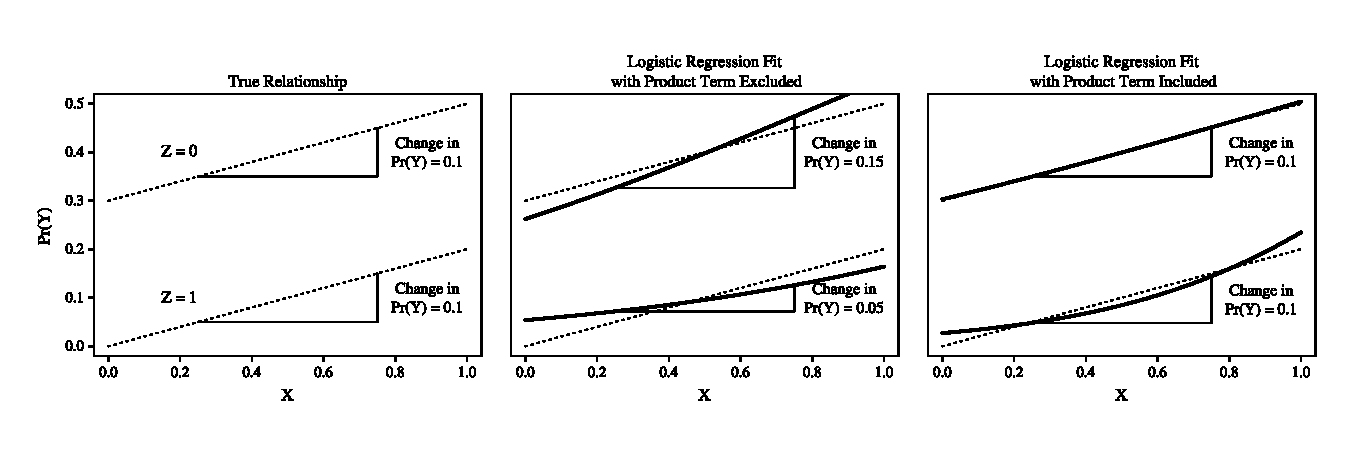
\includegraphics[width=\linewidth]{Figures/fig_example.pdf}
%\vspace{-10mm}
\end{center}
\caption{This figure shows the true relationship in the first simulation study (dotted lines) as well as how logistic regression models with and without a product term fit the process (solid, bold lines). Notice that $X$ and $Z$ have large effects on $\text{Pr}(Y)$ and $\text{Pr}(Y)$ is always less than 0.5. In this case, excluding a product term forces the model to point toward interaction, despite the fact that the relationship is non-interactive. Including a product term allows the model to fit this non-interactive process surprisingly well.}\label{fig:relationships_fits}
\end{figure}

Notice the middle panel of Figure \ref{fig:relationships_fits}, which shows how a logistic regression model without a product term might fit the true relationship. Although there is no interaction in the actual data-generating process, the logistic regression model suggests that there is  substantial interaction between $X$ and $Z$ in influencing $\text{Pr}(Y)$. When $Z=1$, the estimated effect of moving $X$ from 0.25 to 0.75 is 0.05. When $Z=0$, however, the effect of $X$ triples to 0.15 (the second difference is $0.05 - 0.15 = -0.1$). Although the hypothesis of interaction is wrong, the logistic regression model with no product term suggests there is strong evidence in favor of it.

Now notice the right panel of Figure \ref{fig:relationships_fits}, which shows the estimates when the model contains a product term. While this model does not exactly capture the true data-generating process (i.e. notice the non-linearity when $Z = 1$), it estimates the amount of interaction very well. The estimated effect of $X$ when $Z=0$  is 0.1. When $Z = 1$, the estimate is identical. Therefore, the estimated second difference is zero ($0.1 - 0.1 = 0$) and the model correctly suggests that there is no interaction.

Rather than examining how models fit the data-generating process, it is perhaps more informative to evaluate each approach in repeated trials. I simulate 3,000 data sets containing 1,000 observations each. I use each data set to estimate a second difference and its confidence interval using a model with and without a product term. Finally, I estimate the probability of finding interaction when none is present (i.e. a Type-I or false-positive error) by calculating the proportion of data sets that pointed toward interaction with each approach (i.e. the confidence interval does not contain zero). By convention, this probability should be close to 0.05. When the model does not include a product term, the probability of finding interaction is 0.98. This probability  drops to 0.06 when the model includes a product term. 

To help understand why excluding a product term biases the researcher toward finding interaction, Figure \ref{fig:plotted_cis} shows the estimates and confidence intervals from the first 50 simulated data sets, sorted by the size of the estimated second difference. Notice the left panel of Figure \ref{fig:plotted_cis}, which shows that the models without a product term always estimate a substantial amount of interaction in the expected direction  and that the confidence intervals rarely overlap zero. This happens because compression serves as the theoretical motivation for the hypothesis and is \textit{assumed} by the model. But notice the right panel of Figure \ref{fig:plotted_cis}, which shows that most of this bias disappears when a product term is included in the model.

\begin{figure}[h]
\begin{center}
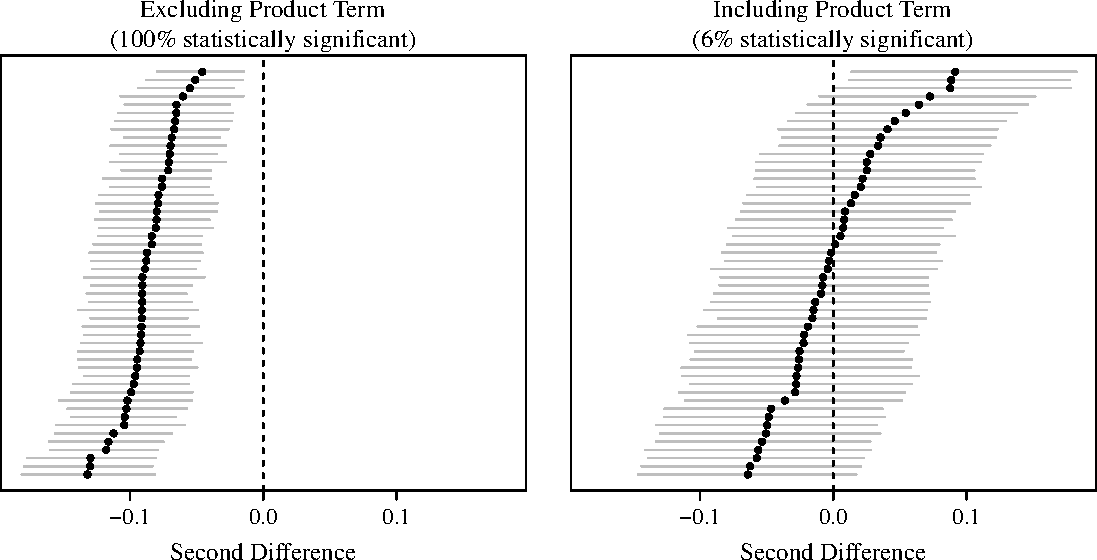
\includegraphics[scale=.7]{Figures/fig_plotted_cis.pdf}
%\vspace{-10mm}
\end{center}
\caption{This figure shows fifty simulations of estimated second differences and confidence intervals using models with and without a product term. Although second difference is actually zero (a non-interactive relationship), the model with no product term consistently finds interaction. Including a product term removes almost all of this bias.}\label{fig:plotted_cis}
\end{figure}

To get a sense of the robustness of this conclusion, I systematically vary the sample size, the distribution of $X$, and the change in $X$ used to calculate the second difference while the true relationship remains the same. For each combination of the simulation parameters, I simulate 3,000 data sets. For each data set, I estimate a logistic regression model with and without a product term and compute the confidence interval around the second difference, as BDE recommend. I then calculate the proportion of simulations in which each model points toward interaction to estimate the probability of finding interaction when none is present. The results are presented in Figure \ref{fig:sm}.

Across all values of the simulation parameters, the models without a product term bias the researcher toward finding interaction and sometimes strongly. The bias is reduced, usually dramatically, when the researcher includes a product term. Indeed, for symmetric distributions of $X$ and centered second differences, adding a product term to the model eliminates nearly all of the bias, lowering the probability of finding interaction
from nearly 1.00 (the worst  situation) to about 0.05 (the ideal situation).

\begin{figure}
\begin{center}
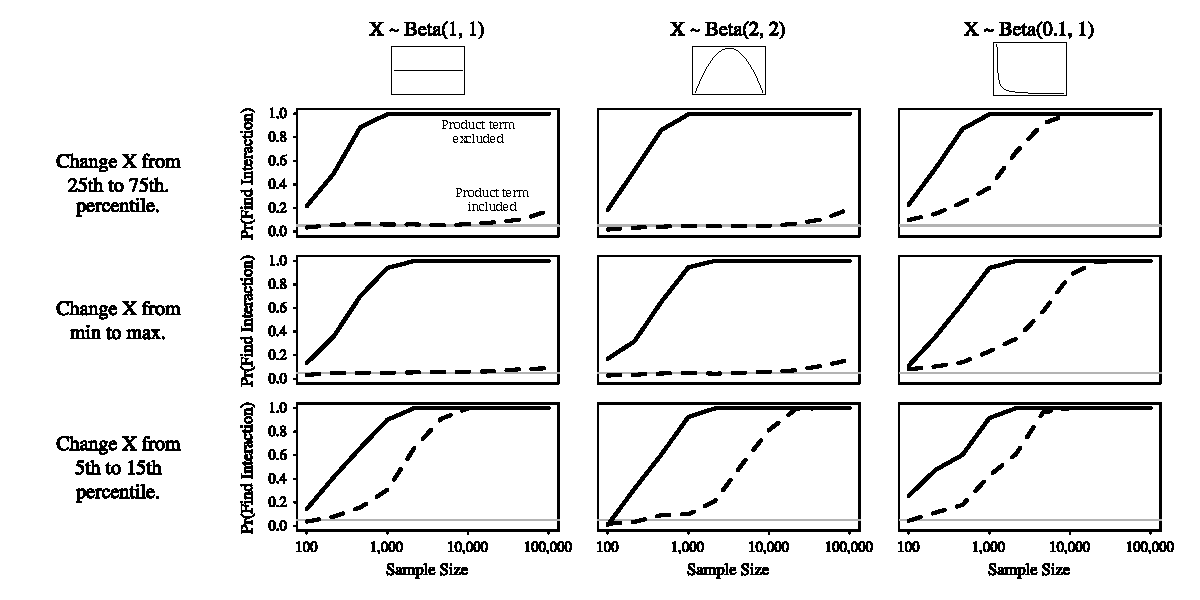
\includegraphics[width=\linewidth]{Figures/fig_sm.pdf}
\end{center}
\caption{This figure shows the probability of concluding interaction when the true relationship is given by $\text{Pr}(Y) = 0.3 + 0.2X - 0.3Z$ (i.e. there is no interaction) using logistic regression models with and without a product term as the sample size, the distribution of $X$, and the change in $X$ considered in computing the second difference varies. Notice that the model including a product term performs remarkably well, although the improvement diminishes as the simple size gets large, especially when the distribution of $X$ is skewed and the researcher considers the effect of changing $X$ nears its extremes.}\label{fig:sm}
\end{figure}

\subsection*{Study \#2: A Diverse Set of Relationships}

To demonstrate that the patterns seen in Figure \ref{fig:sm} do not depend on any particular relationship, I now examine a diverse collection of 1,500 simulated analyses. Each analysis is generated through a random process (described in the Online Appendix) that varies in the following ways:\singlespace\vspace{-3mm}
\begin{enumerate}
\item The relationship between $\text{Pr}(Y)$, $X$, and $Z$ varies, but follows the form of $\text{Pr}(Y) = \beta_0 + \beta_1X + \beta_2Z + \beta_3X^2 + \beta_4Z^2$ and is always monotonic across the range of $X$ and $Z$. Importantly, $X$ and $Z$ never interact in changing $\text{Pr}(Y)$.
\item The distributions of $X$ and $Z$ vary and might be binary, flat, unimodal, or  skewed to the right.
\item The values of $x_{lo}$, $x_{hi}$, $z_{lo}$, and $z_{hi}$ used to construct the second difference vary from zero to one. All combinations are possible, though if a variable is binary, its values are set to zero and one.
\item The sample size varies, ranging from 500 to 100,000, though smaller samples are more likely.


\end{enumerate}
\doublespace
Each ``analysis'' consists of features the researcher totally controls (e.g. values of $x_{lo}$, $x_{hi}$, $z_{lo}$, and $z_{hi}$), somewhat controls (e.g. sample size), and does not control (e.g. distributions of explanatory variables and the true data-generating process). For each simulated analysis, I use the same procedure as before to estimate the probability of finding interaction using models with and without a product term. Because none of the true relationships are interactive, this probability should be near 0.05. 

The left panel of Figure \ref{fig:hist} shows that when the researcher uses a logistic regression model without a product term, the probability of finding interaction when none exists is less than 0.1  for  only 40 percent of the simulated analyses. It is greater than 0.9 for over 20 percent of the analyses. This suggests that excluding a product term biases the researcher toward finding interaction for many plausible relationships. On the other hand, Figure  \ref{fig:hist} also shows that, when using a model with a product term, the probability of finding interaction is less than 0.1  for almost all of the simulated analyses  (over 98 percent).
This suggests that including a product term can eliminate most of the bias toward finding interaction for many plausible relationships and analyses.

\begin{figure}[h]
\begin{center}
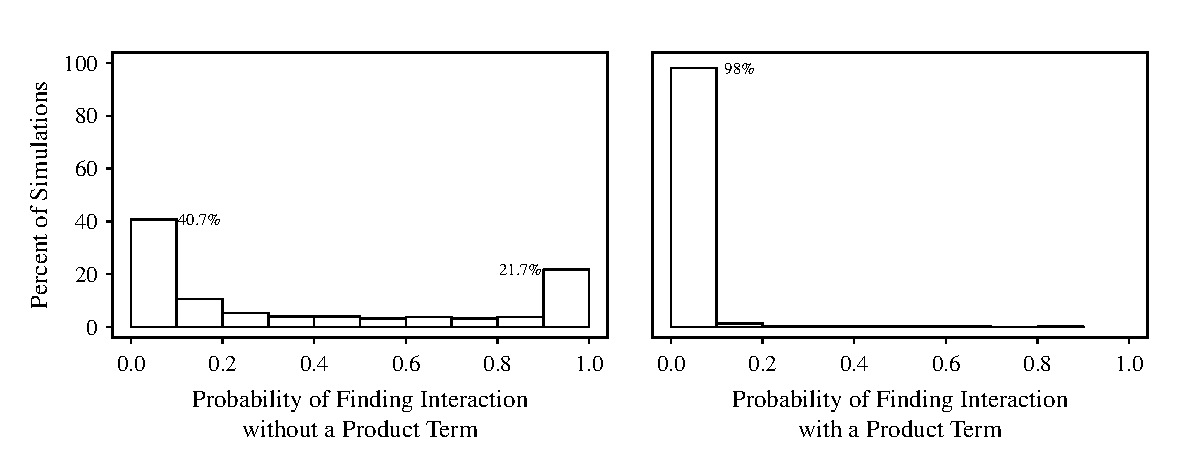
\includegraphics[scale = .7]{Figures/fig_hist.pdf}
\end{center}\caption{The histogram on the left shows that logistic regression models without a product term tend to find interaction when none exists. The histogram on the right shows researchers can eliminate most of this bias by simply including a product term.}\label{fig:hist}
\end{figure}



Figure \ref{fig:scatter} directly compares the two approaches. Notice that every point falls below the diagonal line, which means that the model without a product term is more likely to mislead researchers in \textit{every} simulated analysis. Regardless of the absolute performance of each, the model with a product term clearly improves upon the model without a product term in all the analysis generated in my simulation. In cases in which the model with a product term performs somewhat poorly (e.g. the probability of finding interaction is about 0.3), the model without a product term performs terribly (e.g. the probability of finding interaction is nearly 1.00).
 
\begin{figure}[H]
\begin{center}
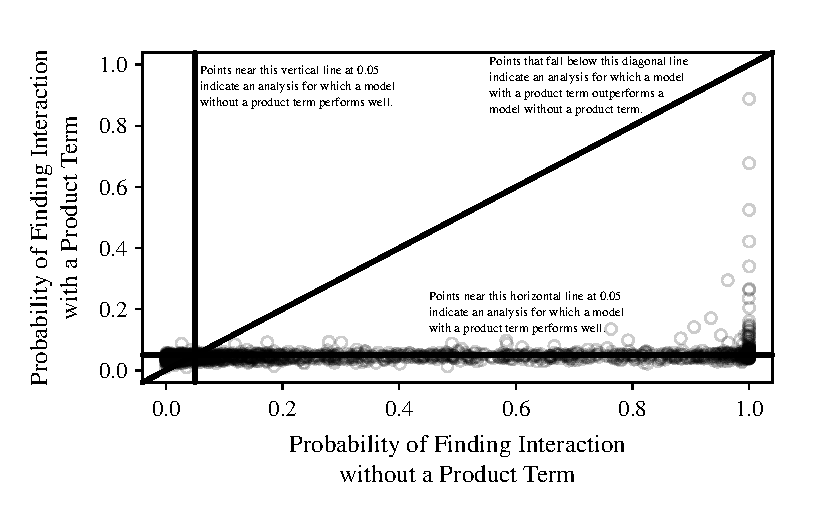
\includegraphics[scale = .9]{Figures/fig_scatter2.pdf}
\end{center}\caption{This figure shows the probability of concluding interaction when none exists from logistic regression models with and without a product term for many different analyses. Notice that many points fall away from the vertical line at 0.05 indicating poor performance of models without a product term. Also notice that most points fall near the horizontal line at 0.05, indicating that models with a product term tend to perform well. Finally, notice that  all points fall below the diagonal line, indicating that models without a product term are more likely to mislead researchers in every simulated analysis.}\label{fig:scatter}
\end{figure}



\section*{Recommendations for Applied Researchers}

I suggest that applied researchers take several steps to ensure their claims of interaction are empirically meaningful.
\singlespace\vspace{-3mm}
\begin{enumerate}
\item Clearly explicate your theory and carefully consider which relationships are consistent and inconsistent with the theory. Only use empirical models that can represent both relationships.
\item As \cite{BerryDeMerittEsarey2010} suggest, specify whether the relevant outcome variable is the latent variable $Y^*$ or the expected value $\text{Pr}(Y)$. If you use the concept $Y^*$, then test for interaction by testing the statistical significance of the product term. If you rely on $\text{Pr}(Y)$, then test for interaction by simulating confidence intervals around a carefully chosen second difference or second derivative. See \cite{BerryDeMerittEsarey2010} and \cite{KingTomzWhittenburg2000} for the details.
\item Regardless of whether the theoretically relevant outcome is $Y^*$ or $\text{Pr}(Y)$, and even if you theorize interaction on the basis of compression alone, you  must include product terms in order to draw compelling substantive conclusions about interaction from logistic regression models. Otherwise, you are simply pulling assumptions through data and treating them as conclusions.
\item As \cite{Nagler1991} notes, if you do not include a product term, then avoid making claims about interaction. The interaction is assumed and you should understand and clearly identify it as such.
\end{enumerate}
\doublespace

\section*{Conclusion}

When researchers are interested in how explanatory variables interact in influencing the probability of an event, my study shows that (1) models \textit{without} a product term point toward interaction very often when none exists, (2) models \textit{with} a product term exhibit much less bias toward interaction, and (3) models \textit{with} a product term almost always reduce and usually eliminate the bias found in models \textit{without }a product term.  Although logistic regression models require ``compression''  to keep the probability of an event bounded between zero and one, researchers can limit the impact of this requirement on tests for interaction by simply including a product term, which allows the models to represent a  broad range of non-interactive relationships surprisingly well. Therefore, even when theorizing interaction due to compression alone, researchers should include a product term, making their theories more vulnerable to the data.\normalsize

\singlespace
\bibliographystyle{apsr_fs}
\bibliography{/home/carlislerainey/Dropbox/Bibliography/bibliography.bib}

\newpage
\begin{appendix}
\singlespace

\begin{center}
\LARGE{\textbf{Online Appendix}}\vspace{4mm}
\end{center}

\section*{Generate a Random Analysis}

\begin{enumerate}
\item Choose a random relationship that is non-linear and non-interactive.
        \begin{enumerate}
        \item Draw $A$ and $B$ from a uniform distribution between 0.3 and 0.7.
        \item Draw $C$ from a uniform distribution between $A$ and $B$ if $A < B$ or between $B$ and $A$ if $B < A$.
        \item Draw $D$ from a uniform distribution between $A - 0.3$ and $A + 0.3$.
        \item Draw $E$ from a uniform distribution between 0 and $D$ if $D > 0$ or $D$ and 0 if $D < 0$.
        \item The true relationship is then given by $Pr(Y) = \beta_0 + \beta_1X + \beta_2Z + \beta_3X^2 + \beta_4Z^2$, where
                \begin{itemize}
                \item $\beta_1 = A$
                \item $\beta_2 = -3A - B + 4C$ 
                \item $\beta_3 = 4E - D$
                \item $\beta_4 = 2A + 2B - 4C$
                \item $\beta_5 = 2D - 4E$ 
                \end{itemize}
        \item Check the resulting relationship is monotonic as $X$ and $Z$ range from zero to one. If not, repeat until a monotonic relationship is obtained.
        \end{enumerate}
        Figure \ref{fig:choose_relationship} illustrates how this procedure works graphically and Figure    \ref{fig:relationship_sample} shows several randomly simulated relationships using this procedure.



        \item Choose a sample size by drawing from a Cauchy distribution, multiplying by 1,000, and rounding to the nearest whole number. The Cauchy distribution has very heavy tails so that most samples fall below 2,000, but very large samples (up to 100,000) occur as well. Table \ref{tab:n} provides the quantiles from this distribution.
        
        \item Choose the distribution of $X$ and $Z$. Perform the following to generate $X$ and $Z$.
                \begin{enumerate}
                \item Choose whether $X$ is binary or continuous. Set as binary with probability 0.5.
                \item If $X$ is continuous, choose the parameters of the Beta distribution from which it will be drawn from a uniform distribution from 0.7 to 3. Figure \ref{fig:distribution_sample}
                \item If $X$ is binary, choose the proportion of ones from a uniform distribution from 0.1 to 0.9.
                \item Repeat for $Z$.
                \end{enumerate}
                
        \item Choose the changes and $X$ and $Z$ used to test for interaction.
                \begin{enumerate}
                \item If $X$ is binary, set $\langle x_{lo}, x_{hi} \rangle$ to $\langle 0, 1 \rangle$.
                \item If $X$ is continuous, then draw and sort two values from a uniform distribution from zero to one. Set these sorted draws as $\langle x_{lo}, x_{hi} \rangle$.
                \item Repeat for $Z$.
                \end{enumerate}
\end{enumerate}

%%% Appendix Figures

\begin{table}[h]
\begin{center}
\begin{tabular}{|cc|}
\hline
Percentile & Sample Size \\ 
\hline
0\% & 500 \\ 
10\% & 646 \\ 
20\% & 815 \\ 
30\% & 1,019 \\ 
40\% & 1,276 \\ 
50\% & 1,614 \\ 
60\% & 2,105 \\ 
70\% & 2,896 \\ 
80\% & 4,427 \\ 
90\% & 8,896 \\ 
100\% & 100,000 \\ 
\hline
\end{tabular}\caption{The distribution of sample sizes I used to simulate analyses.}\label{tab:n}
\end{center}
\end{table}     

        \begin{figure}[h]
        \begin{center}
        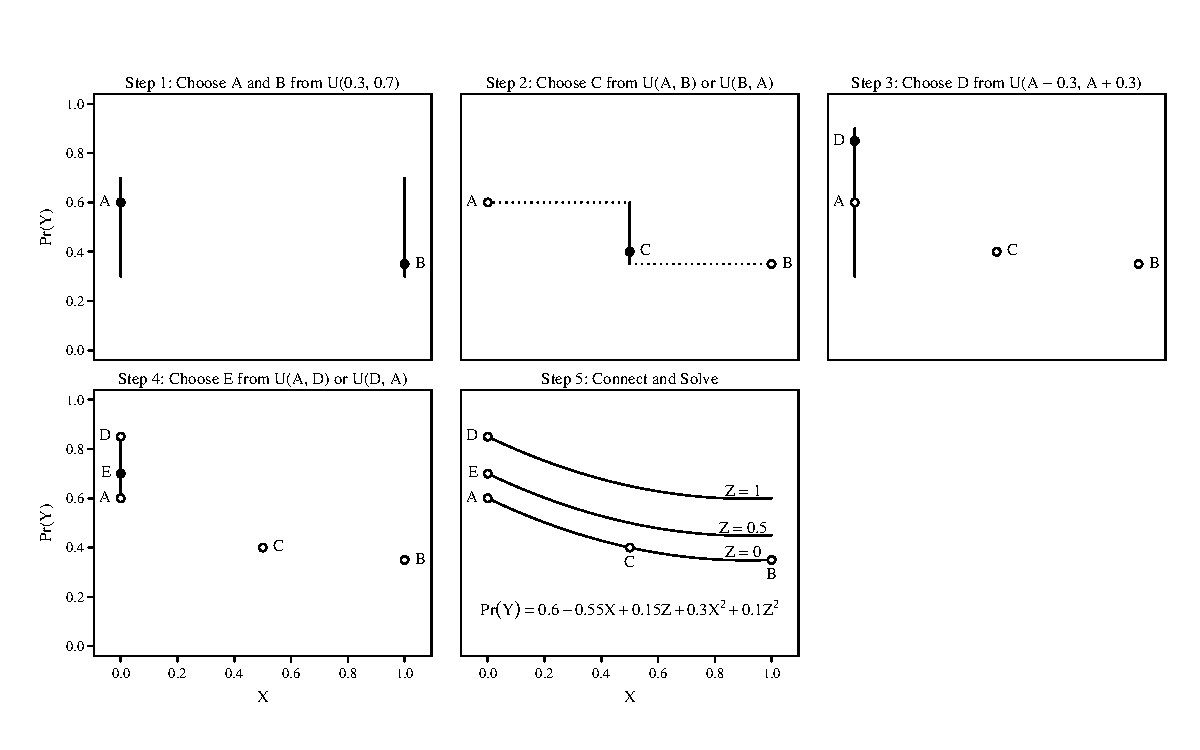
\includegraphics[width = \linewidth]{Figures/fig_choose_relationship.pdf}
        \end{center}\caption{This figure graphically illustrates how I generate random relationships that are non-interactive and non-linear using the procedure describe in Step 1.}\label{fig:choose_relationship}
        \end{figure}
        
 
              \begin{figure}[h]
        \begin{center}
        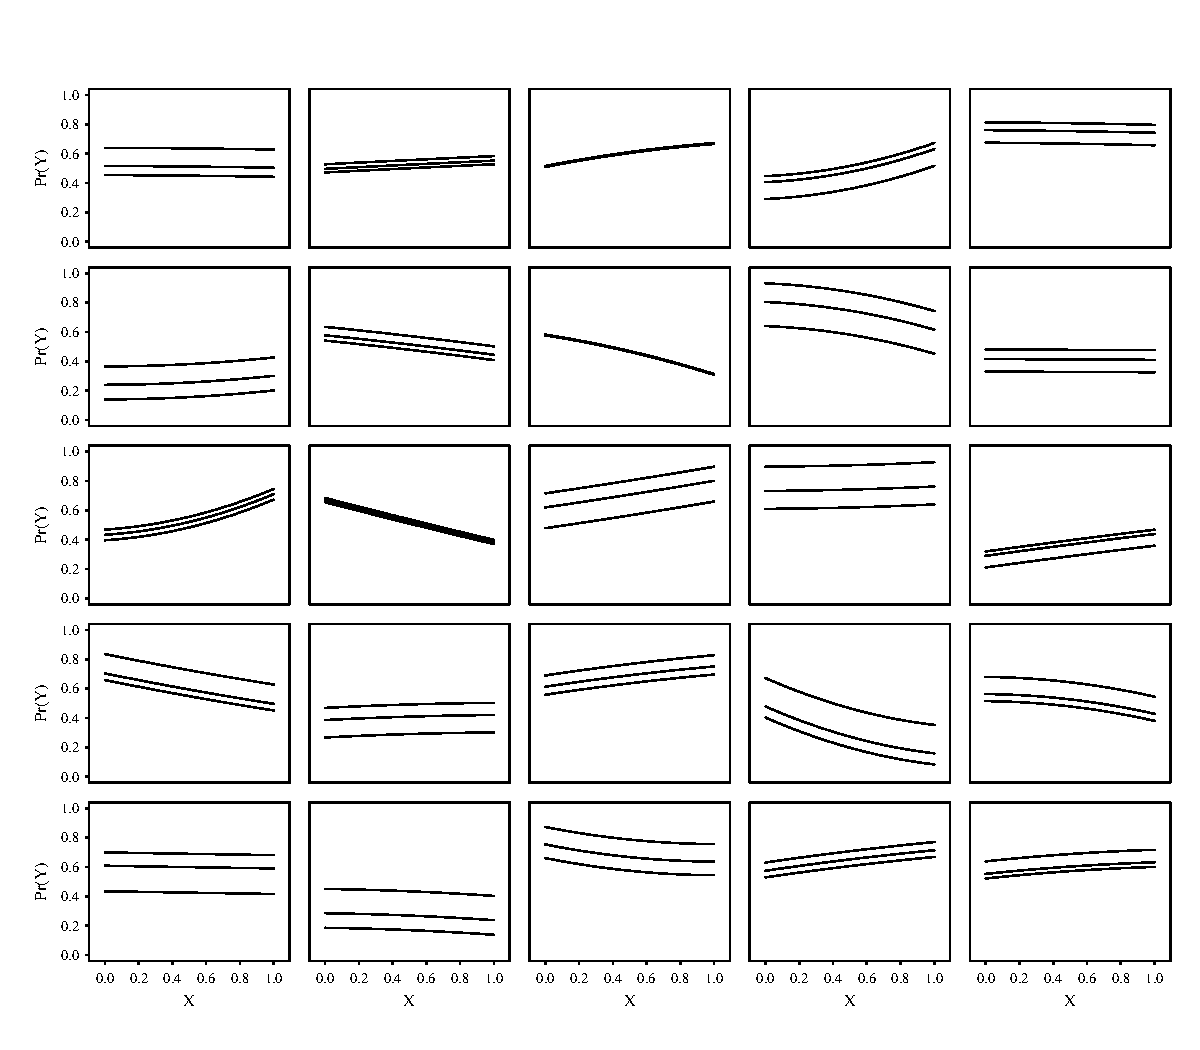
\includegraphics[width = \linewidth]{Figures/fig_relationship_sample.pdf}
        \end{center}\caption{This figure shows several relationships randomly generated using the steps described in Figure \ref{fig:choose_relationship} and Step 1 of the algorithm above. The three lines represent the relationship between $X$ and $\text{Pr}(Y)$ when $Z$ equals zero, one-half, and one, respectively. Due to the assumption of monotonicity described in Step 1(f), the line for which $Z = 0.5$ must fall between the other two.}\label{fig:relationship_sample}
        \end{figure}
        
                                \begin{figure}[h]
        \begin{center}
        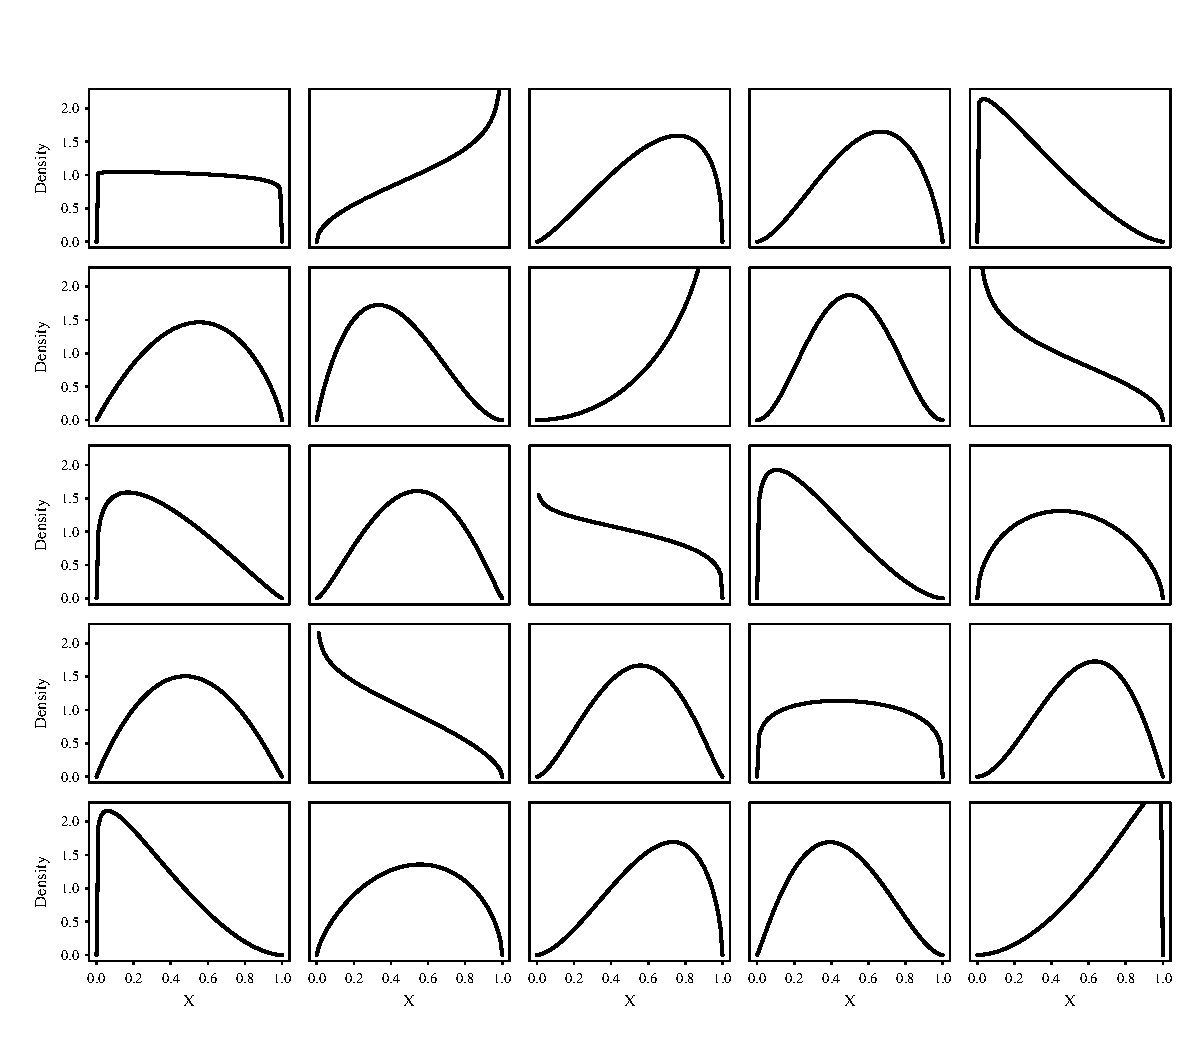
\includegraphics[width = \linewidth]{Figures/fig_distribution_sample.pdf}
        \end{center}\caption{This figure shows several possible continuous distributions of $X$ (or $Z$) randomly generated using Step 3(b). }\label{fig:distribution_sample}
        \end{figure}
        
        
   


\end{appendix}
\end{document}


